\documentclass[a4paper,english,russian]{G2-105}
\usepackage[T1]{fontenc}
\usepackage{listings}
\usepackage{graphicx}
\usepackage{longtable}
\usepackage{booktabs}
\usepackage{standalone}
\usepackage{newclude}
\usepackage[final]{pdfpages}
\usepackage{multirow}
\usepackage{sansmath} % Enables turning on sans-serif math mode, and using other environments
\sansmath % Enable sans-serif math for rest of document
\usepackage[math]{blindtext}

%\usepackage[utf8]{luainputenc}

\begin{document}
%\VSTUAddChapterWordToTOC % обязательно для ПЗ в магистерских диссертациях
\abstract{Аннотация}
\par Документ представляет собой дипломную работу к выпускной работе бакалавра на тему «Продвижение информационных товаров и услуг с применением интернет-маркетинга на примере корпорации Intel», выполненную студентом группы ММОП.м-3.1.3.2, Мельниковым Тимофеем Алексеевичем.
\par В данной работе рассмотрены методы и инструменты интернет-маркетинга, его использование в копропации Intel, а так же эффективность внедрения инструмента интернет-маркетинга Google Analytics в копрорацию Intel.
\par Объём дипломной работы составил составил \totalpages~страниц и включает \totalfigures~рисунков и \totaltables~таблицы. 

\newpage
\par Продвижение информационных товаров и услуг с применением интернет-маркетинга на примере корпорации Intel
%\newpage
\tableofcontents
\newpage

\starchapter{Введение}
\par В настоящее время во всех сферах человеческой жизни происходят значительные изменения. Не является исключением и маркетинг. Сейчас традиционный маркетинг меняется, появляются и создаются новые более востребованные маркетинговые инструменты. Результатом таких изменений можно считать появление интернет-маркетинга. Подавляющая часть потребителей становится активными пользователями сети интернет, что заставило компании переориентировать свою деятельность в интернет-сферу. Смена ориентации деятельности позволяет современным компаниям не только четко выбирать целевую аудиторию, но и эффективно взаимодействовать с нею, минимизируя при этом затраты.
\par Тема использования интернет-маркетинга для продвижения товаров и услуг является актуальной, так как в современном информационном обществе интернет-маркетинг стал наиболее эффективным инструментом привлечения потребителей, продвижения товара и является огромной базой для проведения различных исследований.
\par Объект --- использование сети интернет в маркетинге и применение интернет-маркетинга в корпорации Intel.
\par Предмет --- эффективные технологии и инструменты интернет-маркетинга.
\par Цель дипломной работы --- изучение основ интернет-маркетинга, его методов и инструментов, применение методов в корпорации Intel и анализ рентабельности применения инструмента Google Analytics в компании Intel.
\par В соответствии с поставленной целью мною определены следующие задачи:
\begin{itemize}
	\item Изучить особенности интернет-маркетинга, определить его понятие, цель и функции.
	\item Рассмотреть инструменты интернет-маркетинга, а также его преимущества и недостатки.
	\item Проанализировать использование методов интернет-маркетинга в корпорации Intel.
	\item Показать эффективность внедрения программы Google Analytics на примере корпорации Intel.
\end{itemize}
\par Данная работа состоит из введения, трех глав --- теоретической (Общая характеристика Интернет-маркетинга), аналитической (Использование методов интернет-маркетинга в корпорации Intel) и практической (Применение системы Google Analytics в корпорации Intel).

\newpage

\chapter{Общая характеристика Интернет-маркетинга}
\section{Особенности маркетинга в Интернете}
\par Интернет-маркетинг (англ. internet marketing) - это практика использования всех аспектов традиционного маркетинга в Интернете, затрагивающая основные элементы: цена, продукт, место продаж и продвижение. Основная цель - получение максимального эффекта от потенциальной аудитории.
\par Основные элементы комплекса интернет-маркетинга:
\begin{itemize}
	\item Товар (Product) --- то, что продается с помощью Интернета, должно иметь достойное качество. Он 			конкурирует не только с другими сайтами, но и традиционными магазинами.
	
	\item Цена (Price) --- принято считать, что цена в Интернете ниже, чем в обычном магазине за счет 				экономии на издержках. Контролируйте цены и сравнивайте их с конкурентами регулярно.
	
	\item Продвижение (Promotion) --- комплекс мер по продвижению как сайта, так и товара в целом в сети. 			Включает в себя огромный арсенал инструментов (поисковое продвижение, контекстная реклама, баннерная 			реклама, e-mail маркетинг, вирусный маркетинг, скрытый маркетинг, интерактивная реклама, работа с 				блогами и т.д.).
	
	\item Место продаж (Place) --- точка продаж, то есть сайт. Огромную роль играет как графический дизайн, 			так и юзабилити сайта, и качество обработки заявок с сайта. Так же стоит обратить внимание на скорость 		загрузки, работу с платежными системами, условия доставки, работу с клиентами до, во время и после продажи.
\end{itemize}
\par Интернет-маркетинг является составляющей электронной коммерции. Его также называют online-маркетингом. Он может включать такие части, как интернет-интеграция, информационный менеджмент, PR, служба работы с покупателями и продажи. Электронная коммерция и интернет-маркетинг стали популярными с расширением доступа к интернету и являют собой неотъемлемую часть любой нормальной маркетинговой кампании. Сегмент интернет-маркетинга и рекламы растёт как в потребительском секторе, о чем свидетельствует появление с каждым днем все новых интернет-магазинов. Основными преимуществами интернет-маркетинга считаются интерактивность, который ведет к максимальному повышению таких показателей как конверсия сайта и ROI интернет -рекламы. Интернет-маркетинг включает в себя такие элементы системы как:
\begin{itemize}
\item Gоисковый маркетинг в целом и SEO в частности
\item Продвижение в социальных сетях: SMO и SMM
\item Прямой маркетинг с использованием email, RSS и т.п. [24]
\end{itemize}
\par Основным слагаемым успеха является план маркетинга. Разработанный и внедренный владельцем в любом современном коммерческом предприятии, будь то традиционный магазин или электронный. Потребуются дополнительные маркетинговые мероприятия как в Сети, так и за ее пределами.
\par Забыв о некоторых особенностях пользователей интернета, служащих порой причиной дополнительных ограничений, их культуре и привычной манере общения, можно допустить вторую ошибку, рекламируя свой магазин с помощью рассылки по электронной почте всем, кто только встретится on-line, бесчисленных сообщений о его открытии. Это приведет к широкомасштабному и немедленному "наказанию" со стороны тех пользователей, которые терпеть не могут коммерцию в Сети. Есть, однако, и корректные способы рекламы своего бизнеса в интернете.
\par Надо уметь представить на рынке товары и услуги; необходимо также решить все связанные с этим задачи: сегментирование рынка, определение потребностей потребителей в целевых сегментах и способа продвижения товара, связь с потребителями (другими словами, реклама).
\par Понятие маркетинга в интернете остается наименее изученным и представляет главную проблему фирмы, решившей заниматься коммерцией в этой области. И хотя вряд ли кто-нибудь в ближайшем будущем сможет дать четкое определение данного термина (так как среда пользователей и технология еще не окончательно сформировались), уже сейчас можно предложить несколько стратегий ведения бизнеса в Сети.
\par Интернет создавался не с коммерческой целью, а для обмена информацией между учеными. Но идея ведения бизнеса не чужда ей - она была заложена в самой структуре Сети, хотя привычные для нас красивые названия, такие как "торговые центры", "стендовая реклама", "стратегическое положение", практически ничего не значат в мире электронном. Нехватка новых терминов и обозначений сегодня уже не является временным неудобством в определении маркетинговых подходов, а ставит перед нами вопрос "Что такое маркетинг?", отвечать на который нужно совершенно по-новому.
\par Проблемы маркетинга в интернете. Под маркетингом обычно подразумевается изучение рынка (размеров, демографических характеристик, потребностей) для размещения продукта, определения цены, вероятных покупателей и выработки способов общения с последними. Поэтому человек, занимающийся маркетингом в интернете, обычно сталкивается со следующими проблемами:
\begin{itemize}
\item Неизвестными размерами рынка. О пользователях интернета знаем очень мало. Невозможно, даже более или менее точно определить их число. Наиболее распространенная оценка размера интернета, принадлежащая Internet Society, определяется как число подключенных к сети узловых компьютеров. Вычислить количество пользователей в зависимости от серверов так, чтобы результат соответствовал действительности, практически невозможно. По некоторым оценкам, в настоящее время пользователей Сети порядка 50 миллионов.
\item Пассивностью потребителей. Достаточно ли знать, что потребителей "много" и "их число растет". Как правило (имеется в виду разновидности бизнеса), точные цифры --- "сколько" и "как быстро" - не нужны. В конце концов, расходы на подключение к интернету по сравнению с затратами на открытие настоящего магазина и оплату труда работников относительно невелики.
\par Настоящие проблемы возникают, когда вы пытаетесь сообщить (неизвестно кому!) о своем существовании и продукции. Сегодняшние возможности передачи данных - электронная почта и доски объявлений (телеконференции) --- абсолютно неприемлемы для распространения такой информации. Необходимо четко понимать, что товары и услуги нельзя рекламировать в Сети так же, как по телевидению, то есть прямо и настойчиво. Предложения своих услуг, продукции в подобной форме и явное продвижение самого себя не поощряются. Нарушение неписаных правил немедленно приводит к реакции со стороны пользователей --- нарушителя "сжигают", иными словами, ему посылают тысячи осуждающих сообщений по электронной почте. Огромный объем информации способен вывести из строя сеть пользователя, которая окажется не в состоянии справиться с обработкой такого количества сообщений. Это отобьет у нарушителя всякое желание иметь дело с интернетом. Пользователи могут также объявить бойкот товарам и услугам компании и вообще перестать связываться с ней по Сети. И уж совсем редко, но все же случается и такое, что нарушителю лично доставляют массу беспокойства телефонными звонками часа в два ночи домой, звонками на работу.
\par Например, при создании крупнейшей американской коммерческой сети учитывалась возможность подобных операций. Однако, пройдя и через рекламу, и через "торговые центры", компания изменила структуру получения доходов, когда выяснилось, что пользователям нужно, скорее, средство общения, нежели возможность совершать покупки в режиме online. А в некоторых случаях --- таких как торговля цветами или программным обеспечением --- дела шли как нельзя лучше. Так что успех предприятия в интернете зависит не столько от умения торговца правильно подать себя, сколько от того, окажутся ли полезными его товары или услуги для пользователей.
\par Существует множество объяснений, почему некоторые электронные магазины терпят неудачу (здесь не учитывается явные недостатки: плохой пользовательский интерфейс, нехватки графики, неудобного механизма оформления заказов, невозможности оплаты наличными и так далее). Однако, как правило, поведение покупателей обуславливается следующими моментами:
\begin{enumerate}
\item привычки: "Обычно я делаю покупки (хлеб, одежду и так далее) совсем не так";
\item несоответствие цели: "Я сюда не за этим пришел";
\item неизвестность: "Я не знаю, что там было, --- я искал только то, что хотел найти";
\item несовершенство систем поиска: "Мне был нужен видеомагнитофон, но я не собирался просматривать десять разных магазинов".
\end{enumerate}
\par По сравнению с обычными средствами массовой информации - газетами, телевидением и радио, - которые, по сути, предназначены для передачи коммерческих сообщений, интернет довольно пассивен в смысле проведения маркетингового комплекса. Вы просто делаете вывеску и ждете посетителей.
\item Незнание потребителей. Если разобрались с незнанием реальных объемов рынка сбыта и потребительской пассивностью, то что сказать о маркетинге, основанном на достигнутых результатах и обратной связи с покупателями. Другими словами, не достаточно ли определить один раз маркетинговые мероприятия и проводить их, основываясь на собственном опыте, пусть и небольшом. Можно не изменять, не адаптировать политику маркетинга, рекламу, основанную лишь на отзывах посетителей.
\par В отличие от пассивной, нисходящей на потребителя модели маркетинга, интернет позволяет осуществить взаимодействие поставщиков и потребителей, при котором последние сами становятся поставщиками (в частности, поставщиками информации о своих потребностях).
\end{itemize}
\par Поскольку интернет представляет собой совершенно новую коммуникационную среду в отличие от традиционных средств информации, во многих случаях некоторые приемы и средства маркетинга не могут быть применены в их существующей форме.
\par При рассмотрении модели, использующей для рекламы традиционные средства массовой информации, оказывается, что использование интернета дает возможность потенциальным клиентам не выступать в роли пассивной аудитории, а самостоятельно принимать решение, следует ли им знакомиться с конкретной рекламной информацией. Таким образом, интернет трансформирует функцию маркетинга.
\par При работе в интернете фирма, раскрывая и удовлетворяя потребности клиента, должна стремиться внести свой вклад в разработку новых идей и методов для электронной коммерции.
\par Таким образом, новая роль маркетинга помимо удовлетворения потребностей клиента непосредственно включает в себя "альтруистическую", кооперативную цель облегчения развития рынка.
\section{Основная цель интернет-маркетинга}
\par Интернет-маркетинг появился в начале 1990-х годов, когда текстовые сайты начали размещать информацию о товарах. Сейчас интернет-маркетинг --- это нечто большее, чем продажа информационных продуктов, сейчас идет торговля информационным пространством, программными продуктами, бизнес-моделями и многими другими товарами и услугами. Такие компании, как Google, Yahoo, и MSN подняли на новый уровень и сегментировали рынок интернет-рекламы, предлагая малому и среднему бизнесу услуги по локальной рекламе. Рентабельность инвестиций возросла, а расходы удалось снизить. Этот тип маркетинга стал основой современного капитализма, которая позволяет любому, у кого есть идея, товар или услуга, достичь максимально широкой аудитории. Использование термина "интернет-маркетинг" обычно подразумевает использование стратегий маркетинга прямого отклика, которые традиционно используются при прямых почтовых рассылках, радио и в телевизионных рекламных роликах, только здесь они применяются к бизнес пространству интернета. Эти методы оказались очень эффективными при использовании в интернете благодаря возможностям точно отслеживать статистику, умноженным на возможность находиться в относительно постоянном контакте с потребителями. Эта возможность анализа применяется сейчас повсеместно, и поэтому так часто можно увидеть такие термины, как ROI --- коэффициент окупаемости инвестиций, conversion rate --- коэффициент эффективного посещения (он же - конверсия сайта), а также мгновенно получить статистику продаж, спроса и т.д. [24]
\par Основная цель интернет - маркетинга - это получение максимального эффекта от потенциальной аудитории. Условно, все инструменты интернет-маркетинга можно разделить на две группы:
\begin{itemize}
\item Поисковый маркетинг, куда относятся поисковое продвижение сайта, контекстная реклама.
\item Не поисковый маркетинг, куда можно отнести медийную рекламу, вирусный маркетинг, маркетинг в социальных сетях, PR в интернете.
\end{itemize}
\par Отдельно стоит упомянуть веб-аналитику, которая показывает, насколько эффективно работает маркетинг, окупаются ли средства вложенные в продвижение и многое другое. Интернет-маркетинг, как комплекс мер по работе с сайтом выходит за рамки собственно привлечения трафика на сайт. Это не просто продвижение сайта, это уже продвижение бизнеса в сети интернет. Весь комплекс работ в рамках интернет-маркетинга имеет три основные цели:
\begin{itemize}
\item информирование аудитории о услугах/продукте, его преимуществах;
\item вызвать интерес к услуге/продукту;
\item "подтолкнуть" заинтересовавшихся к покупке.
\end{itemize}
\par Добиться реализации всех трех целей, путем отдельно взятой рекламной компанией или тематическим продвижением --- чрезвычайно сложно, а вот сочетая все доступные инструменты и возможности --- реально. Всю работу по продвижению бизнеса в интернете можно условно разделить на следующие этапы:
\begin{enumerate}
\item Знакомство с бизнесом. На этом этапе проводится различного рода исследования. Необходимо понять, что и кому будем предлагать, определить характеристики продукта и компании, целевую аудиторию и конкурентное окружение. На этом же этапе идет изучение истории проекта: что делалось ранее и что делается сейчас, какие цели ставились и какие результаты получены.
\item Подготовка к продвижению. На этом этапе планируется компания по продвижению: определение методов и способов продвижения, аудит сайта, расчет бюджета, определение всех необходимых работ по подготовке сайта, определение основных показателей эффективности работы сайта, рекламных компаний. Внедрение и настройка инструментов веб-аналитики.
\item Подготовка к продвижению. На этом этапе планируется компания по продвижению: определение методов и способов продвижения, аудит сайта, расчет бюджета, определение всех необходимых работ по подготовке сайта, определение основных показателей эффективности работы сайта, рекламных компаний. Внедрение и настройка инструментов веб-аналитики.
\item Формирование отчетности, анализ эффективности, внесение изменений в план действий. С самого начала ведется контроль эффективности предпринимаемых мер и действий, что позволяет во время сфокусировать внимание на проблемных участках и в конечном итоге - добиваться всех поставленных целей.
\end{enumerate}
\section{Интернет-маркетинг и традиционный маркетинг: сходства и различия}
\par Использование Интернета привносит новые особенности и преимущества по сравнению с маркетингом, основанном на традиционных технологиях. Вот некоторые из них:
\begin{itemize}
	\item Переход ключевой роли от производителей к потребителям.
\par Одним из наиболее фундаментальных качеств, привнесенных интернетом в мир современной коммерции, является переход ключевой роли от производителей к потребителям. Интернет сделал реальностью для компаний возможность привлечь внимание нового клиента всего за десятки секунд, проведенных им перед экраном компьютера. Однако в то же время он дал возможность тому же пользователю за несколько щелчков мыши перейти к любому из конкурентов. В такой ситуации внимание покупателей становится самой большой ценностью, а установленные взаимоотношения с клиентами главным капиталом компаний.
	\item Глобализация деятельности и снижение транзакционных издержек.
\par Интернет значительно изменяет пространственный и временной масштабы ведения коммерции. Он является глобальным средством коммуникации, не имеющим каких-либо территориальных ограничений, при этом стоимость доступа к информации не зависит от удаленности от нее, в противоположность традиционным средствам, где эта зависимость прямо пропорциональна. Таким образом, электронная коммерция позволяет даже самым мелким поставщикам достигать глобального присутствия и заниматься бизнесом в мировом масштабе. Соответственно, заказчики также получают возможность глобального выбора из всех потенциальных поставщиков, предлагающих требуемые товары или услуги независимо от географического расположения. Расстояние между продавцом и покупателем играет роль лишь с точки зрения транспортных издержек уже на этапе доставки товаров.
\par Временной масштаб в интернете также значительно отличается от обычного. Высокая эффективность коммуникативных свойств интернета обеспечивает возможность сокращения времени на поиск партнеров, принятие решений, осуществление сделок, разработку новой продукции, и т. д. Информация и услуги в интернете доступны круглосуточно. Кроме того, его коммуникативные характеристики обладает высокой гибкостью, позволяющей легко производить изменения представленной информации, и, тем самым, поддерживать ее актуальность без временной задержки и затрат на распространение.
\par Названные эффекты также приводят к значительному сокращению транзакционных издержек, то есть издержек, связанных с налаживанием и поддержанием взаимодействия между компанией, ее заказчиками и поставщиками. При этом стоимость коммуникаций, по сравнению с традиционными средствами, становится минимальной, а их функциональность и масштабируемость значительно возрастают.
\item Персонализация взаимодействия и переход к маркетингу "один-одному".
\par Используя средства электронного взаимодействия, компании могут получать подробную информацию о запросах каждого индивидуального заказчика и автоматически предоставлять продукты и услуги, соответствующие индивидуальным требованиям. Одним из простых примеров может служить персональное представление web-сайта для каждого из клиентов или партнеров компании.
\par В результате интернет позволяет перейти от массового маркетинга к маркетингу "один-одному". В таблице ~\ref{am} приведены данные по сравнению характеристик массового маркетинга с маркетингом "один-одному".
\begin{longtable}{|c|c|}
    \caption{Сравнение массового маркетинга и маркетинга "один-одному"}\\ \hline
    \label{am} 
    Массовый маркетинг & Маркетинг "один к одному" \\ \hline \endhead
    Усредненный покупатель & Отдельный покупатель \\ \hline
    Анонимность покупателя & Характеристики покупателя \\ \hline
    Стандартный продукт & Специальное маркетинговое предложение \\ \hline
    Массовое производство & Специальное производство \\ \hline
    Массовое распределение & Индивидуальное распределение \\ \hline
    Массовая реклама & Индивидуальное обращение \\ \hline
    Массовое продвижение & Индивидуальные стимулы \\ \hline
    Одностороннее обращение & Двусторонние обращения \\ \hline
    Масштабная экономика & Целевая экономика \\ \hline
    Доля рынка & Доля покупателей \\ \hline
    Все покупатели & Потенциально прибыльные покупатели \\ \hline
    Привлечение покупателей & Удержание покупателей \\
\end{longtable}
\item Снижение трансформационных издержек
\par Снижение трансформационных издержек может достигаться за счет оптимального выбора структуры товарного ассортимента, сокращения времени на разработку и внедрение новой продукции, обоснованной политики ценообразования, снижения числа посредников, затрат на сбыт и т.д.
\par Например, одним из способов снижения трансформационных издержек может быть сокращение каналов распространения товаров. Причиной сокращения каналов распространения является возможность для фирм взять на себя функции, традиционно выполняемые специалистами промежуточных звеньев, так как интернет обладает более эффективной возможностью взаимодействия с потребителями и одновременно позволяет отслеживать информацию о потребителях.
\par Особый случай --- продукты и услуги, которые могут быть доставлены электронным способом. При этом путь доставки сокращается максимально. Электронный способ широко применяется для доставки цифровых продуктов индустрии развлечений (фильмы, видео, музыка, журналы и газеты), информации, средств обучения и эффективно используется компаниями, занимающимися разработкой и поставкой программного обеспечения.
\end{itemize}
\section{Преимущества и ограничения интернет - маркетинга}
\par Интернет-маркетинг в первую очередь предоставляет потребителю возможность получить информацию о товарах. Любой потенциальный потребитель может, используя интернет, получить информацию о товаре, а также купить его. Хотя, если там не будет информации об одном товаре, или он её не найдёт, то, скорее всего он приобретёт другой товар у конкурента.
\par Применение методов интернет-маркетинга нацелено на экономию средств (на заработной плате сотрудников отделов продаж и на рекламе), а также на расширение деятельности компаний (переход с локального рынка на национальный и международный рынок). При этом как крупные компании, так и малые, имеют более уравновешенные шансы в борьбе за рынок. В отличие от традиционных рекламных медиа (печатных, радио и телевидения), вход на рынок через интернет является не слишком затратным. Важным моментом является то, что в отличие от традиционных маркетинговых методов продвижения, интернет-маркетинг дает чёткую статистическую картину эффективности маркетинговой кампании.
\par В сравнении с другими видами медиамаркетинга (печатными, радио и телевидением), интернет-маркетинг растет очень быстро. Он завоёвывает все большую популярность не только у бизнеса, но и обычных пользователей, которые хотят продвинуть свой эффективный веб-сайт или блог и заработать на нем. Тем не менее, в развитых странах, затраты на интернет-маркетинг и рекламу составляют около 5\% от общих рекламных затрат.
\par Следующее неудобство состоит в том, что интернет-маркетинг не дает возможность потребителю опробовать товар до того, как сделать покупку. Но большинство потребителей решают эту проблему просто. Они знакомятся с интересующим их товаром в обычном магазине, а покупку делают в интернет-магазине. Германия, например, приняла в 2000 году закон (Fernabsatzgesetz, позже объединён с BGB), по которому любой покупатель может вернуть товар, купленный через интернет без всяких объяснений и получить полный возврат денег. Это одна из основных причин, почему в Германии так развита интернет-торговля.
\par Проблема отсутствия возможности у покупателя "потрогать" товар также может решаться иными способами, например, некоторые владельцы интернет магазинов используют фотографии товара высокого качества и разрешения, стараясь передать в изображениях все детали и особенности своей продукции. Набирает популярность и использование специальной фото-техники для оцифровки снимков товара в формате 3D (объемное изображение), дающее посетителю интернет магазина рассмотреть товар со всех ракурсов
\section{Влияние интернет маркетинга на бизнес}
\par Интернет-маркетинг оказал огромное влияние на ряд деловых сфер, включая музыкальную индустрию, банковское дело, рынок портативных электронных устройств (мобильные телефоны, плееры и т.д.), так называемый "блошиный рынок" и главное --- на рекламу.
\par В музыкальной индустрии на данный момент жесткие носители потеряли свое доминирующее место. Музыкальные произведения доступны онлайн, на удаленных серверах.
\par Интернет-маркетинг также повлиял и на банковскую индустрию. Онлайн-банкинг является более удобным для клиента, так как избавляет от необходимости посещать каждый раз банк или его филиалы. В США на сегодняшний день большинство людей пользуются услугами онлайн-банкинга. Онлайн-банкинг является одним из наиболее быстрорастущих секторов интернет-бизнеса. Увеличивающиеся скорости интернет-соединений занимают в этом исключительно важную роль. Из всех пользователей Интернета около 70\% пользуются услугами интернет-банкинга.
\par Интернет-аукционы завоевали популярность, блошиные рынки борются за выживание. Уникальные вещи, которые раньше можно было найти на блошиных рынках, теперь продаются на онлайн-аукционах, таких как eBay. Также развитие аукционов сильно повлияло на цены на уникальные и антикварные вещи. Если прежде информацию о цене найти было трудно, то теперь можно посмотреть цену на аналогичную вещь на аукционе. И иметь хотя бы общее представление о стоимости товара, так как всегда можно узнать, за сколько продавалась та или иная вещь. Все больше и больше продавцов подобных товаров ведут свой бизнес онлайн, сидя дома.
\par Эффект на рекламную индустрию был и остается поистине огромным. В течение всего нескольких лет объем онлайн-рекламы стремительно вырос и достиг десятков миллиардов долларов в год. Рекламодатели начали активно менять свои предпочтения и сегодня интернетреклама уже занимает большую рыночную нишу, чем реклама на радио (в развитых странах).
\par На сегодняшний день сложно найти крупное индустриальное предприятие, которое не продвигает себя в сети. Тенденции роста можно легко увидеть и по постоянному расширению торговых интернет-площадок, а также росту их количества. Торговые онлайн-площадки уже давно перестали быть досками объявлений, из которых они и выросли. Сегодня некоторые из них превратились в крупные корпорации, предоставляющие целый ряд маркетинговых услуг. Растут и цены за участие на таких площадках (имеется в виду привилегированное членство), несмотря на то, что количество их увеличивается.
\section{Проблемы интернет-маркетинга в России}
\par Главными объективными препятствиями на пути становления маркетинга в России стали супермонополизм в промышленности, диктат централизованного ценообразования, дефицит товаров и неготовность кадров к работе в многовариантном, многополюсном, взаимозависимом мире. Все это консервировало несвободу выбора как для покупателей, так и во многом для производителей товаров и услуг. В таких условиях потенциал маркетинга не мог быть реализован, за исключением отдельных шагов па уровне отдельных фирм, организаций.
\par Субъективными факторами, тормозившими развитие маркетинга, стали распространенные в нашем обществе антимаркетинговые стереотипы (психологические установки и подходы) в восприятии маркетинга сo стороны хозяйствующих субъектов и граждан, либо неоправданно упрощавшие его понимание и процедуры осуществления, либо наоборот, излишне усложнявшие и приводившие к отказу от его использования целые сферы экономики - малый бизнес, некоммерческие виды деятельнoсти и др. Эти стереотипы в значительной степени не преодолены и до сих пор.

\newpage

\chapter{Использование методов Интернет – маркетинга в корпорации Intel}
\section{Общая информация о корпорации Intel}
\par Американская корпорация, производящая широкий спектр электронных устройств и компьютерных компонентов, включая микропроцессоры, наборы системной логики (чипсеты) и др. Штаб-квартира — в городе Санта-Клара, штат Калифорния, США.
\par Компанию основали Роберт Нойс и Гордон Мур 18 июля 1968 года после того, как ушли из компании Fairchild Semiconductor. Вскоре к ним присоединился Энди Гроув.
Компания Intel является сегодня крупнейшим производителем полупроводников в мире. Она изменила наш мир не меньше, чем это сделали Apple и Microsoft в свое время (а если говорить точнее, то они ничего бы не сделали без Intel). Ведь Intel изобрела микропроцессор – сердце современных компьютеров. В начале XXI века процессоры Intel были установлены более чем на 80\% компьютеров по всему миру. Сегодня Intel выпускает достаточно широкий спектр продукции, который не заканчивается на одних лишь процессорах. Так, компания производит материнские платы, флэш-память, концентраторы и маршрутизаторы, концептуальные ноутбуки и многое другое [5].
\par Корпорация Intel на протяжении многих лет известна во всем мире как один из лидеров в сфере высоких технологий. Чтобы идти в ногу со временем и в течение длительного времени возглавлять бурно развивающуюся индустрию, необходимо не только проводить научные исследования и уникальные конструкторские разработки, но также постоянно искать новые пути построения маркетинговых коммуникаций с конечными потребителями.
\section{Применение методов интернет-маркетинга в корпорации Intel}
\par Для Intel целевой аудиторией являются, во-первых, специалисты в области информационных технологий. При чем это не только IT-менеджеры, принимающие решения, но и IT-профессионалы в общем. Эта часть аудитории характеризуется достаточно высокой квалификацией, она постоянно работает с компьютерами и стремятся быть в курсе последних технологических разработок в силу не только личной любознательности, но и служебных обязанностей.
\par Вторую и большую часть целевой аудитории составляют продвинутые пользователи. Это активная публика, не всегда хорошо подкованная в техническом плане, но стремящаяся знать как можно больше о лучших новинках и получить личный опыт пользования ими.
\par При этом и первая, и вторая группа целевой аудитории отличается прагматичным подходом к информации и открыта к eё получению. Также, общим для всей целевой аудитории является постоянное интенсивное пользование компьютерами. Решение о переносе мeдийных компаний в онлайн было принято Intel больше 10 лет назад. Если у большинства компаний на долю интернета приходится от 5 до 10\% общего мeдийного бюджета, то Intel делает основной акцент именно на развитии интернет-сообщества.
\par Конечно, сделано это по вполне прагматичной причине. Как уже говорилось, интернет является основным источников информации для целевой аудитории Intel и самым прямым и коротким путём общения с нею.
Однако недостаточно просто найти нужный канал коммуникации. Используя то или иное медиа, приходится учитывать его особенности. Поиск в нем нужных и, главное, достоверных сведений --- задача непростая и часто не находящая своего решения.
\par Традиционная баннерная реклама, хотя и обладает рядом преимуществ по сравнению с «медиа прошлого века» (например, доступность статистики), тем не менее, имеет и множество недостатков. В целом надо признать, что баннерная реклама чаще всего не воспринимается аудиторией, чему в немалой степени способствует тот факт, что современные браузеры позволяют отменить eе загрузку на веб-страницах.
\par Поэтому для максимально эффективного использования 100\% медийного бюджета Intel следовало ориентироваться на другие каналы коммуникаций, обеспечиваемые интернетом. Итак, в онлайн-продвижении было решено сделать упор на том, что всемирная паутина является интерактивной средой, предоставляя компаниям уникальную возможность вступать в прямой диалог со своими потребителями.
\par Именно по этой причине в качестве наиболее эффективной альтернативы традиционной интeрнет-рeкламе стали рассматриваться социальные сети. На данный момент ими пользуется более 90\% всех посетителей Рунета, что, безусловно, делает эти ресурсы мощным инструментом маркетинга. Однако, работая с социальными медиа, необходимо учитывать региональную специфику их аудитории. Централизованное управление маркетинговыми проектами в данной области практически невозможно и, как минимум, неэффективно. Демографический профиль аудитории крупнейших международных социальных сетей значительно разнится от региона к региону. Сильнее выражены отличия в предпочтениях и поведении пользователей.
\par Поэтому успешные проекты в социальных сетях были придуманы и организованы именно в российском представительстве Intel.
\par В июне 2007 года в социальной сети LiveJournal было создано сообщество i\_future, посвящённое информационным технологиям и их влиянию на будущее. Блоковая основа LiveJournal стала оптимальной платформой для реализации маркетингового проекта Intel, направленного на взаимный обмен пользователей информацией.
\par Сегодня i\_future, объединяя более 8300 пользователей, занимает первую строчку среди технических сообществ в LiveJournal. У проекта достаточно продвинутая аудитория, активно интересующаяся многими темами не только в ЖЖ, но также в других проектах и сетях. Благодаря этому наиболее интересные темы блогеров i\_future часто обсуждаются за пределами самого сообщества. Как следствие, нередки попадания в независимые рейтинги самых обсуждаемых блогов Рунета.
\par Характерная черта i\_future --- широкий тематический охват. Это буквально все, что касается сегодняшних и завтрашних технологий и разработок, а далеко не только продукты и решения от самой Intel. Современная архитектура и градостроительство, экология и «зеленные технологии», дизайн и концептуальные прототипы, научные исследования и новости из лабораторий, экономика и, конечно, IT --- все это обсуждается в сообществе. Доля контента, генерируемого при участии Intel, не превышает 30\%. Также в сообществе публикуется информация от партнёров, но основная часть контента создаётся в настоящее время уже усилиями самих блогеров --- участников сообщества.
\par Однако самым массовым проектом Intel в социальных сетях стала группа «Галактика Intel», появившаяся в сети «ВКонтакте» в ноябре 2008 года. Сегодня она насчитывает порядка 70 тыс. участников и является крупнейшей hardware-группой этой сети. Аудитория «ВКонтакте» очень сильно отличается от той, которая собрана компанией в сообществе i\_future. Она значительно моложе и слабее подготовлена в техническом плане, что не мешает ей активно интересоваться компьютерными новинками. Разумеется, с точки зрения маркетинга, аудитория, охватываемая сетью «ВКонтакте», также очень важна для Intel.
\par Участники группы интенсивно обсуждают специфические для eе состава темы, советуются друг с другом. Предоставление им информации в основном ведётся через комментируемую новостную ленту. Здесь также присутствует много партнёрской информации, проводятся конкурсы с призами.
\par Два проекта в области социальных сетей Intel развернула весной 2008 года непосредственно на своём российском сайте --- это «Галактика Intel» (Intel Galaxy) и IT Gаlаxy. Первый ориентирован на более широкую потребительскую аудиторию и связан с одноимённой группой «ВКонтакте». Второй является сообществом IT-профессионалов и органично дополняет аудиторию остальных социальных сетей.
\par Ключевая особенность аудитории проектов Intel Galaxy и IT Galaxy --- высокая степень доверия к бренду. На этих площадках компания периодически проводит различные активности в рамках программы лояльности, такие, например, как игра IT Manager III, позволяющая зарабатывать баллы, которые затем можно обменять на ценные призы. Эта игра представляет собой симулятор работы IT-специалиста. Сначала он управляет IT-отделом в небольшой компании, решает проблемы с техникой, обучает персонал. По мере развития компании увеличивается количество задач, растёт численность его отдела, появляются удалённые офисы. Новые проблемы приходится решать быстро, в рамках бюджета. Причём достичь наилучшего результата в игре позволяет применение технологий Intel. Основная задача игры: демонстрация возможностей современных технологий Intel в корпоративной игровой среде, максимально приближенной к реальной жизни. Например, последние обновление игры включает в себя сценарий «всемирного экономического кризиса», когда бюджет IT-отдела резко сокращается и его руководителю приходится решать вопрос: обосновать руководству необходимость получения дополнительного финансирования или работать в имеющихся условиях. Стоит отметить тот факт, что игроки из России входят в ТОП-20 мирового рейтинга (общее количество игроков в мире: более 58000, в России: более 8000).
\par При ориентации на совершенно разную аудиторию, Intel Galaxy и IT Galaxy имеют схожую структуру, основными компонентами которой служат:
\begin{itemize}
\item активно комментируемый новостной блог;
\item традиционный по формату форум;
\item конкурсы;
\item опросы.
\end{itemize}
\par На рисунке ~\ref{diagram1} показана диаграмма с процентным соотношением пользователей в описанных выше социальных проектах. Противовес в сторону группы Intel Galaxy понятен, в виду ориентации на массового пользователя.
\par Есть и специальные проекты, такие как «Клуб экспертов» на Intel Galaxy или «Лаборатория Intel» на IT Galaxy, которые дают членам сообществ различные привилегии. Например, «Лаборатория Intel» предоставляет возможность IT-профессионалам протестировать самое новое оборудование на базе технологий Intel. Техника установлена в лаборатории Intel в Нижнем Новгороде, любой желающий может записаться на консультацию, в рамках которой ему будет предоставлен удалённый доступ с возможностью загрузки своего ПО для тестирования и консультации специалистов Intel. Также в сообществе IT Galaxy любой желающий может пройти IT Galaxy IQ Test[5]. В режиме онлайн на экране в формате чата появляются вопросы на общие темы, а также на знание продуктов и новостей компании Intel. Победителем становится зарегистрированный участник, давший правильный ответ быстрее всех. Лучшие игроки становятся лидерами своеобразного рейтинга «умников» и получают призовые баллы в рамках программы лояльности Intel.
\begin{figure}
    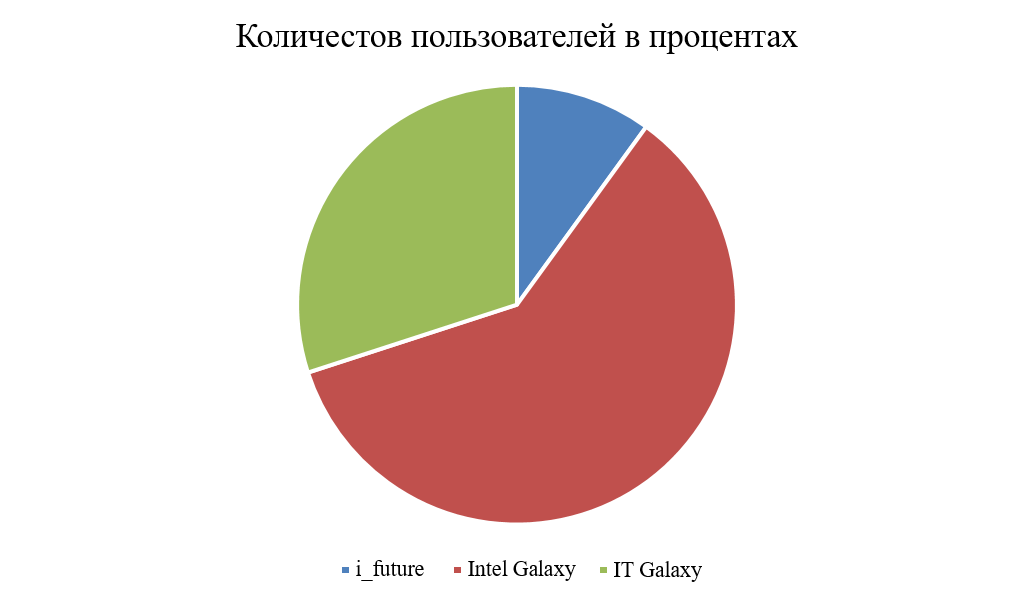
\includegraphics[width=\linewidth]{diagram1.png}
    \caption{Количество пользователей в разных сообществах корпорации Intel}
	\label{diagram1}
\end{figure}
\section{Анализ SMM деятельности корпорации Intel}
\par Аудитория сообществ, сформировавшихся на данный момент вокруг сайта www.intel.ru, довольно велика (на IT Galaxy, например, зарегистрировано свыше 34 тыс. человек), что дат возможность использовать эти проекты в качестве площадки для экспериментов. После удачной обкатки в максимально лояльных и в то же время требовательных сообществах, новшества переносятся в другие проекты.
\par Уникальность проектов Intel Galaxy и IT Galaxy состоит также в предоставлении участникам этих сообществ возможности общаться с сотрудниками компании в оперативном онлайновом режиме. Сегодня постоянные блоги в этих проектах ведут более 10 инженеров и специалистов Intel. Получение информации «из первых рук», ответы на вопросы и участие в обсуждениях высококвалифицированных профессионалов – это действительно важные достоинства социальных сетей Intel.
\par В отличие от проектов в сетях «ВКонтакте» и LiveJournal, Intel Galaxy и IT Galaxy в большей степени концентрируются на технологиях и продукции Intel. Благодаря этим площадкам компании удалось сформировать своего рода базу знаний по этим вопросам, открытую для обсуждений, динамично пополняющуюся новыми публикациями, отслеживающую реальные интересы и потребности аудитории.
\par Привлечение новых участников в сообщества Intel Galaxy и IT Galaxy идет по нескольким основным направлениям:
\begin{itemize}
\item Через поисковые системы Рунета. При запросе, релевантном содержанию этих проектов, пользователь может обнаружить ссылки на Intel Galaxy или IT Galaxy в результатах поисковой выдачи и, перейдя по ним, оценить, насколько ему интересен такой контент.
\item Как уже говорилось, на эти сообщества идет прямая ссылка с корпоративного сайта компании www.intel.ru. Таким образом, любой заинтересованный посетитель сайта может стать участником сообщества.
\item Во время проведения различных конкурсов и викторин на крупнейших IT-площадках Рунета едет анонсирование этих мероприятий. Желающий принять участие в розыгрыше может перейти на сайт и зарегистрироваться в сообществе.
\item Также многие представители целевой аудитории регистрируются в сообществе по приглашению своих друзей и знакомых, уже являющихся членами IT Galaxy. Всем участникам, друзья которых зарегистрировались в сообществе и стали eе активными членами, начисляются призовые баллы в рамках программы лояльности.
\end{itemize}

\par Правом вносить свои темы для обсуждения в сообществе обладают все зарегистрированные пользователи. Здесь также работает система поощрений: авторы самых интересных материалов и полезных комментариев получают «баллы» в рамках программы лояльности Intel, которые затем могут обменивать на призы.
\par Обратившись к социальным сетям, Intel к настоящему времени построила надёжно работающий канале для двусторонних коммуникаций с конечными потребителями своих технологий и продуктов. Благодаря использованию разных по демографии и профессиональному составу сообщества этот эффективный инструмент маркетинга охватывает все важные для компании части целевой аудитории — от рядовых потребителей до IT-менеджеров, принимающих решения.
\par Интернет, независимо от внешних условий, развивается динамично. Появляются новые способы коммуникаций, открывающие принципиально новые, ранее неизвестные медийные возможности [6, с. 187]. Поэтому для успешного маркетинга в интернете любой компании нужно постоянно держать руку на пульсе событий, проявляя креативность и не боясь выйти за пределы традиционных подходов.
\par Результаты проделанной работы корпорации Intel по привлечению клиентов, используя интернет-маркетинг приведены в таблице ~\ref{money}. В ней показана валовая прибыль корпорации, полученная использованием интернет-маркетинга.
\begin{longtable}{|c|c|c|c|c|}
    \caption{Валовая прибыль от интернет-маркетинга корпорации Intel}\\ \hline
    \label{money} 
    Год & 2014 & 2015 & 2016 & 2017 \\ \hline
    Валовая прибыль, млн. \$ & 2,006 & 2,049 & 2,158 & 2,104 \\ \hline
\end{longtable}

\chapter{Применение системы Google Analytics в Intel}
\section{Характеристика программы Google Analytics}
\par Сайт в интернете представляет собой инструмент для продвижения определенного товара или вида услуг: будь то конкретный товар или ваши мысли о том, как его лучше продать.
\par Конечно же, как и любой продукт, сайт требует конкретной оценки своей эффективности.
С этой целью более 6 лет назад компанией Urchin Software было разработано программное обеспечение для анализа статистики посещения и трафика сайтов в сети интернет.
\par В апреле 2005 года компания Google выкупила Urchin Software Corporatoins, чтобы использовать этот продукт для определения эффективности своих рекламных проектов. В результате внедрения новых программ и настроек, Urchin был усовершенствован и в 2006 году получил название Google Analytics. Начиная с августа 2006 года, сервис Google Analytics стал доступен для всех желающих. И сегодня, по оценке агентства инновационного маркетинга Promo Interactive, Google Analytics является наиболее популярным инструментом статистики взаимодействия интернет-пространства и его пользователей Analytics (сокращённо GA) - бесплатный сервис, предоставляемый компанией Google для создания детальной статистики посетителей веб-сайтов. Статистика собирается на сервере Google, пользователь только размещает JS-код на страницах своего сайта.
\par Бесплатная версия ограничена 5 миллионами просмотров страниц в месяц. Пользователям с активным аккаунтом Google Ad Words предоставляется возможность отслеживания неограниченного числа просмотров страниц. Особенностью сервиса является то, что вебмастер может оптимизировать рекламные и маркетинговые кампании Google AdWords при помощи анализа данных, полученных при помощи сервиса Google Analytics, о том откуда приходят посетители, как долго они остаются на сайте и где они находятся географически.
\par Сервис интегрирован с Google AdWords. Пользователи видят группы объявлений и отдачу от ключевых слов в отчётах. Также доступны дополнительные возможности включая разделение посетителей на группы.
\par Пользователи сервиса могут определить цели и последовательности переходов. Целью может выступать страница завершения продаж, показ определённых страниц, или загрузка файлов. Используя данный инструмент, маркетологи могут определять, какая из рекламных кампаний является успешной, и находить новые источники целевой аудитории.
\par Любой пользователь может добавить до 50 профилей сайтов. Каждый профиль обычно соответствует одному сайту Analytics показывает основную информацию "на панели инструментов", более детальную информацию можно получить в виде отчёта. В данный момент доступно 80 видов настраиваемых отчётов.
\par Благодаря настройке RSS, можно отслеживать переходы по соответствующей ссылке. При этом расположение ссылок не важно - это могут быть тексты, реклама и даже картинки. Важно знать, как анализировать информацию по целям. Для этого нужно обратить внимание на левое меню. Специалисты советуют, что если кликов было 300, эту цифру следует делить на два, так как кто-то кликнул по ошибке, а кто-то из любопытства, то есть фактическое количество кликов уменьшается. Analytics представляет собой бесплатный сервис, с помощью которого можно получить детальную статистику посетителей любого сайта. Для этого достаточно на каждой странице сайта установить соответствующий код JavaScript (JS-код). У любого пользователя есть возможность добавить до 50 профилей сайтов, и в бесплатном варианте осуществлять до 5 миллионов просмотров страниц в месяц.
\par Статистика Google Analytics позволяет выяснить, с какой страницы интернета пришли посетители на ваш сайт, где они расположены в это время географически и сколько времени они находились на вашем сайте.
\par Данные Google Analytics эффективно используются оптимизаторами для законной раскрутки сайтов. Умелое их применение способствует продвижению сайта и достижению результатов показов на первых страницах поисковых систем.
\par Помимо основной информации, при помощи дополнительных настроек в Google Analytics можно получить более 80 видов отчетов, например, таких как статистика переходов по ссылкам и анализ поведения пользователей при работе с сайтом.
\begin{figure}
    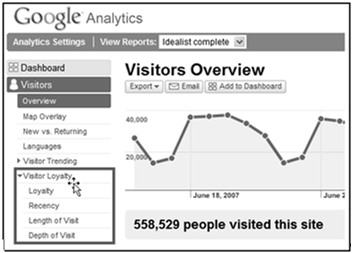
\includegraphics[width=\linewidth]{ris1.png}
    \caption{Показатели Google Analytics}
	\label{ris1}
\end{figure}
\par При анализе статистики Google Analytics важно четко различать основные его показатели:
\begin{itemize}
\item Уникальные посетители - это неповторяющиеся (учитываемые только один раз) посетители Вашего сайта за указанный период времени. Уникальным считается посетитель, зашедший на ваш сайт с одного IP-адреса.
\item Сеанс посетителя - это период взаимодействия между браузером посетителя или вашим сайтом, который завершается при закрытии окна браузера, завершении работы браузера или неактивности пользователя на сайте на протяжении 30 минут.
\item Сеансы возврата - это количество возвращений на Ваш сайт уникальных посетителей за указанный период времени.
\end{itemize}
\par Уникальные посетители формируют рейтинг вашего сайта, и, помимо проявления заинтересованности в предлагаемом вами продукте, делают сайт привлекательным для рекламодателей.
\par Итак, в первую очередь нужно определиться, что можно делать при помощи этой программы.
\par Значительные преимущества Google Analytics:
\begin{itemize}
\item можно отслеживать статистику переходов на сайт;
\item классифицировать посетителей (такой подход позволяет разрабатывать новые страницы сайта целенаправленно);
\item можно отслеживать исходящие ссылки, используемые при продвижение сайта, что также необходимо для дальнейшей раскрутки сайта;
\item можно отслеживать ссылки, которые скачивают больше всего;
\item можно отследить адреса электронной почты по кликам;
\item практически все коммерческие транзакции прослеживаются при помощи этого программного обеспечения;
\item можно также отключить статистику посещений тех, кто обслуживает сайт;
\item можно сравнить статистики посещения сайта за разные периоды (данная возможность идеальна для выявления эффективности работы новых страниц).
\end{itemize}
\par Недостатки у Google Analytics все же есть:
\begin{itemize}
\item отследить трафик в случае, если у пользователя отключены cookies файлы невозможно;
\item кроме того, Google Analytics не может повторно обработать данные, если потерян профиль с настроенными фильтрами;
\item настройка отчетов имеет ограниченное количество (в частности можно настроить до 12 разных отчетов);
\item количество отслеживаемых целей также ограничено (в настоящее время Google.Analytics отслеживает до четырех целей. К слову, каждая цель может быть конвертирована для получения дополнительной прибыли).
\end{itemize}
\section{Краткое описание работы в Google Analytics}
\par Для регистрации нового аккаунта или входа в систему, нужно зайти на официальный сайт Google: www.google.com/intl/ru/analytics/ далее действовать согласно инструкциям.
\par Если уже есть аккаунт в любом из сервисов Google (GMail, AdWords, Adsense и т.п.), то регистрироваться заново не обязательно. Только если не хотите иметь отдельный аккаунт для Google Analytics. Не будем подробно останавливаться на процессе регистрации, потому что там все просто.
\par Настройка профиля сайта (рис.3.2.) в аккаунте Google Analytics: чтобы данные обрабатывались правильно, надо настроить профиль сайта. В текущем окне, справа от названия профиля, нажать на ссылку "Изменить", и откроются настройки этого профиля:
\begin{figure}
    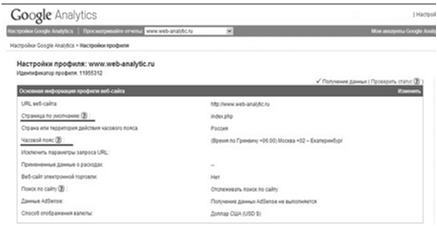
\includegraphics[width=\linewidth]{ris2.png}
    \caption{Настройка профиля Google Analytics}
	\label{ris2}
\end{figure}
\par Здесь главное правильно указать "Страницу по умолчанию" - это главная страница сайта (обычно index.php или index.html). И правильный часовой пояс. Оба этих параметра влияют на данные в отчетах.
Рассмотрим еще одну страницу- это "Панель инструментов" (Рисунок ~\ref{ris3}).
\begin{figure}
    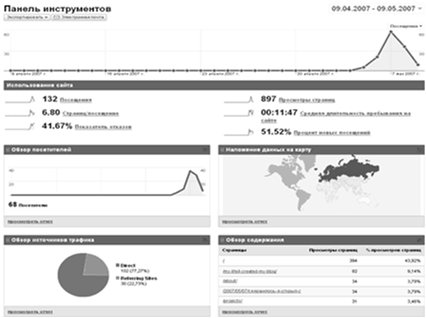
\includegraphics[width=\linewidth]{ris3.png}
    \caption{Панель инструментов Google Analytics}
	\label{ris3}
\end{figure}
\par Данная страничка представляет собой "краткое содержание" системы, по умолчанию это:
\begin{itemize}
\item График посещений
\item Использование сайта
\item Обзор посетителей
\item Наложение данных на карту
\item Обзор источников трафика
\item Обзор содержания
\end{itemize}
\par Если что-то не нужно на этой панели - вы можете удалить отчет, или добавить другой, можете поменять расположение элементов, в общем удобно.
\par Глядя на график можно заметить, что первые посетители пришли на сайт 5-го мая. Подобный график будет "преследовать" практически на каждой странице статистики. Далее рассмотрим страницу "Обзор посетителей" (Рисунок ~\ref{ris4})
\begin{figure}
    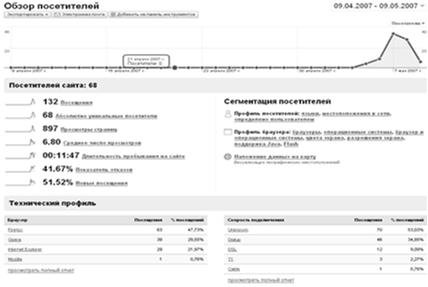
\includegraphics[width=\linewidth]{ris4.png}
    \caption{Обзор посетителей Google Analytics}
	\label{ris4}
\end{figure}
\par Первая страничка раздела "Посетители" предоставляет общую информацию без ненужной детализации.
\par Источники трафика --- это раздел для тех кто занимается раскруткой сайтов, первая страничка "Обзор" соответствует своему названию:
\begin{figure}
    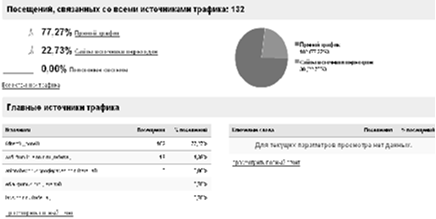
\includegraphics[width=\linewidth]{ris5.png}
    \caption{Источники трафика Google Analytics}
	\label{ris5}
\end{figure}
\par Далее есть много подпунктов данного раздела:
\begin{itemize}
\item Прямой трафик --- статистика пришедших по URL введенному вручную в браузере (или тех кому отправили ссылку по какому-либо мессенджеру).
\item Сайты-источники переходов --- оставили ссылку на сайт где-то на просторах Интернета - вот и пришли гости.
\item Поисковые системы --- кто-то что-то искал, а нашёл именно этот сайт.
\item Все источники трафика --- результирующая страничка по предыдущим трём.
\item Ключевые слова --- когда ктото ищет этот сайт в поисковиках и по какому слову нашел этот сайт. Данный пункт предназначен для работы с AdWords.
\item Кампании --- тут перечислены кампании AdWords, почему не подпунктом AdWords.
\item Версии объявлений --- работа с объявлениями AdWords.
\end{itemize}
\par Содержание - еще один не маловажный пункт статистики, можно просмотреть какие разделы сайта наиболее интересны пользователям, и какие наиболее популярные точки выхода (Рисунок ~\ref{ris6}).
\begin{figure}
    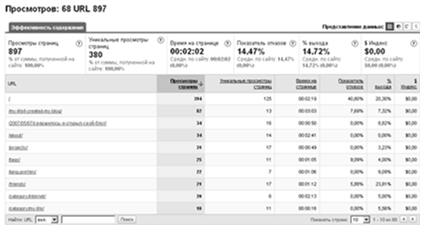
\includegraphics[width=\linewidth]{ris6.png}
    \caption{Обновление данных "Google Analytics"}
	\label{ris6}
\end{figure}
\section{Эффективность внедрения программы Google Analytics на примере Intel}
\par Проведение анализа поведения пользователей на сайте - необходимая часть внедрения проекта в Интернете. И чем проект сложнее и разветвленнее, чем крупнее.
\par С помощью Google Analytics грамотный специалист сможет определить основные аспекты поведения посетителя на сайте и его seo блог всегда будет посещаем и доступен в первых рядах поисковой выдачи. Он будет знать сколько времени пользователь провел на сайте, какие страницы посещал, и с каких он покинул сайт.
\par Однако, это не значит, что начинающему блогеру не нужно заглядывать и разбираться с данными аналитики.
\par Результатом работы Google Analytics является предоставление файла с отчетом, в котором представлена вся информация о посещаемости, сделаны выводы, и дальнейшие рекомендации по улучшению сайта. Скачивайте данные отчеты себе на компьютер, и периодически возвращайтесь, сравнивайте с новыми значениями, обязательно отмечая проделанную работу и какие она повлекла результаты
\par Компании Intel удалось оптимизировать свой сайт на основании отчетных данных Google Analytics с помощью функции наложения данных на сайт Google Analytics и отчетов, показывающих, что компания теряет почти половину клиентов. Компания сократила процесс до одного шага и свели его на одну страницу, поэтому количество посетителей увеличилось на 50\%. По прогнозам, это будет способствовать значительному росту доходов в ближайшие несколько месяцев. Продолжает тестировать и контролировать программы маркетинга в интернете с помощью веб-аналитики. До Google Analytics инетрнет-компания тратила маркетинговый бюджет, главным образом, наугад. Теперь, зная, в какой мере кампании окупаются и насколько они эффективны, система Google Analytics оказала большое положительное воздействие на бизнес фирмы.
\par Возьмем в качестве примера показатели статистики сайта Intel. Согласно данным, представленным Google Analytics, за период с 1 мая 2015 года по 1 мая 2016 года, сайт посетили 2 202 000 посетителей, из которых 1 066 000 - уникальных.
\par Физическое местонахождение посетителей сайта Inte; зафиксировано в 37 странах мира, из которых: 81\% процента посетителей сайта из Америки, Китай - 9\%, остальная часть распределена между странами Европы и Средней Азии. Сравнивая эти показатели, можно выявить процент популярности сайта на определенной территории, в данном случае - в Америке.
\par Точно также, пользуясь статистикой Google Analytics, а также необходимыми для сравнения данными, можно определить для своего сайта: территориальное размещение заинтересованных посетителей, процент посетителей вашего сайта в общем количестве пользователей и другие важные показатели.
\par При этом важно иметь в виду, что количество посещений отражает не только потребность в вашем продукте, но и эффективность работы вспомогательных служб вашей компании - маркетологов и веб-мастеров.

\starchapter{Заключение}
\par Коммерческое использование Интернета, в значительной степени связанное с появление и развитием службы World Wide Web, насчитывает менее чем одно десятилетие, однако за этот небольшой промежуток времени произошло громаднейшее число самых разнообразных событий, рождение большого числа новых компаний. Обороты рынка электронной коммерции за это время выросли во много раз и скоро достигнут отметки в \$ трлн. Компаниям Интернет предоставил новый инструмент ведения бизнеса, средство снижения издержек и более полного удовлетворения потребностей потребителей. Потребители, в свою очередь, получили новый информационный источник о товарах и услугах, новые пути удовлетворения своих потребностей за счет возможности взаимодействия с более широких кругом компаний и новое эффективное средство коммуникации, как с компаниями, так и между собой.
\par Этот период зарождения электронного бизнеса выявил два важных момента. Во-первых, Интернет доказал свою высокую эффективность, как средства коммуникации, и высокий потенциал построенного на его основе глобального электронного рынка. Во-вторых, опыт компаний, либо пытающихся использовать Интернет, как дополнение своего традиционного (off-line) бизнеса, либо изначально построивших свой бизнес в Интернете, подтвердил важность и необходимость учета и использования всего существующего опыта по ведению коммерческой деятельности и использованию принципов маркетинга в своей деятельности.
\par Наряду с бурным ростом электронного бизнеса одним из важных явлений стало появление нового направления в маркетинге - интернет-маркетинга. В некоторых источниках это направление также именуется как гипермаркетинг, в котором приставка гипер- подчеркивает гипермедийный характер среды Интернета. Все эти названия объединяет та сущность, которая лежит в основе глобальной компьютерной Сети - это гипер- и мультимедийная глобальная компьютерная среда предоставляющая невиданные до сих пор возможности взаимодействия, начиная от простого обмена информацией, кончая осуществлением финансовых транзакций, заключением сделок и доставкой цифровых продуктов.
\par В сегодняшней коммерческой практике весьма интенсивно используется Интернет. В ходе проведенного исследования установлено, что интенсивность использования интернет-технологий в предпринимательской практике возрастает. Большинство коммерческих структур, фирм организаций и учреждений с помощью технологий Интернета успешно осуществляют коммерческие операции. Интернет на современном этапе развития предпринимательства выступает как специфический элемент развития рыночной инфраструктуры. Система Интернета позволяет создавать и распределять информационные потоки, формировать бизнес-сообщества (интернет-компании). По сути Интернет создает предпосылки для формирования специфического сектора бизнеса.
\par Результаты работы над данным дипломным исследованием позволяет установить, что использование интернет-технологий создает предпринимателям несколько важных направлений повышения эффективности бизнеса: ускорение процесса платежных операций, повышение оперативности коммунальных связей, использование Интернета, как дополнительного канала информационных потоков.
\par Во-первых, на фоне бурно развивающегося и изменяющегося Интернета темпы преобразований в областях маркетинга и рекламы в Сети впечатляют. За последние годы и в мире, и в России Интернет-реклама стала заметным и самостоятельным бизнесом. Но в силу того, что российский Интернет далеко не во всем похож на Интернет Европы и США, и реклама в нашем Интернете существенно отличается от рекламы в иных странах, полноценное использование Интернета как маркетингового инструмента в России только начинает зарождаться.
\par Во-вторых, Интернет дает множество инструментов для воздействия на целевую аудиторию при проведении рекламных кампаний. Среди них можно выделить: размещение рекламы на тематических и общеинформационных сайтах, баннерные сети, e-mail маркетинг, продвижение с помощью поисковых систем и каталогов, обмен ссылками, рейтинги и т.д.
\par Но помимо приведенных способов интернет-рекламы, наличие самого сайта рекламодателя является обязательным условием при проведении рекламных кампаний.
\par Компания, имеющая свой сайт и занимающаяся рекламой в Интернете имеет ряд преимуществ перед традиционной рекламой: более низкая стоимость рекламной кампании по сравнению с традиционными СМИ; большая аудитория, чем у СМИ; возможность направления потока рекламы только на целевую аудиторию; возможность таргетинга рекламных кампаний в зависимости от портрета целевой аудитории; возможность оперативного управления рекламными кампаниями; возможность оценки эффективности рекламы более качественной, чем у традиционных СМИ.
\par В-третьих, интернет-реклама - это высоко технологичное средство коммуникаций, которое позволяет в ходе рекламной кампании собирать данные о количестве показов рекламных баннеров, отслеживать нажатия на баннеры, но самой удобной возможностью является то, что можно оперативно менять баннеры, которые имеют низкий отклик на более эффективные, тем самым корректирую рекламную кампанию в течение всего периода.
\par Наконец, исследование всех теоретических и прикладных аспектов позволяет разобрать методику анализа и оценки эффективности рекламных кампаний с использованием Интернета.
\par По завершению рекламной кампании подводятся итоги, собираются и анализируются данные, которые в последствии требуется изучить и получить информацию о том, на сколько эффективно прошла рекламная кампания, что следует учесть при следующих рекламных кампаниях, нужно ли продолжать рекламную кампанию вообще.
\par Данные для анализа предоставляются системами статистики, необходимо иметь доступ к статистике сайта или баннерной сети, где происходит реклама, а также иметь собственную статистику сайта.
\par Делая вывод - Google.Analytics многофункциональный сервис, который позволяет осуществлять раскрутку сайта более эффективно. Для этого важно научиться пользоваться панелями инструментов этого программного обеспечения. Конечно, минусы у Google.Analytics все же есть, но они при всех преимуществах незначительны. Именно поэтому, многие сегодня пользуются этой программой для отслеживания трафика на своем сайте, исключая неэффективные методы раскрутки в самом начале работы.

\newpage
\begin{thebibliography}{1}
	\bibitem{1} Амблер Т. Практический маркетинг / Т. Амблер. - СПб.: Питер, 1999. - 400 с.
\bibitem{2} Багрин Ю. Интернет как новый маркетинговый канал // Маркетинг и реклама. 2009. -- № 1. 2.
\bibitem{3} Бокарев Т.А. Способы продвижения компании в сети Интернет// Маркетинг и маркетинговые исследования в России, 2009. - № 4.
\bibitem{4} Бурдинский А.А. Интернет-маркетинг как новый инструмент развития бизнеса// Маркетинг и маркетинговые исследования в России, - 2005. - № 2.
\bibitem{5} Бушуева Л.И. Роль Интернет-услуг в практической маркетинговой деятельности // Маркетинг в России и за рубежом №4, 2001 г.
\bibitem{6} В. Холмогоров. Интернет-маркетинг. Краткий курс. - Питер, 2002 г., с: 272
\bibitem{7} Голик В.С. Эффективность Интернет-маркетинга в бизнесе. -Дикта, 2008 г., с: 196
\bibitem{8} Голубков Е.П. Использование Интернета в маркетинге // Маркетинг в России и за рубежом №3 (29), 2002 г.
\bibitem{9} Гуров В. Интернет для бизнеса. -М.:Дело, 2006. -289 с.
\bibitem{10} Данько Т.П. Управление Интернет-маркетингом: Учебное пособие.- М.: Инфра-М, 2007.
\bibitem{11} Закарян И., Филатов И. Интернет как инструмент интернет-маркетинга. -СПб.:BHV, 2006. - 302 с.
\bibitem{12} Интернет-маркетинг на 100 \%. -Питер, 2009 г., с: 240
\bibitem{13} Колесников О.Э. Интернет для делового человека. -М.:МЦФ. Издат. Фирма Яуза, 2004 -281 с.
\bibitem{14} Михайлова Е.А. Проблемы и перспективы взаиморазвития Интернета и международного маркетинга // Маркетинг в России и за рубежом, 2003. - №6.
\bibitem{15} Михаил Зуев, Денис Разваляев. Интернет-маркетинг. Взгляд практиков. - Вершина, 2008 г., с: 248
\bibitem{16} Панкрухин А.П. Маркетинг: учебник для студентов.- М.: Омега Л,2007
\bibitem{17} Пол Гринберг. CRM со скоростью света. Привлечение и удержание клиентов в реальном времени через Интернет. - Символ-Плюс, 2006 г., с: 530
\bibitem{18} Пименов Ю.С. Использование Интернет в системе маркетинга//Маркетинг в России и за рубежом. -2003. -№1. -с. 2-5.
\bibitem{19} Успенский И.В. Интернет-маркетинг Учебник.- СПб.: Изд-во СПГУЭиФ, 2003 г.
\bibitem{20} Филипп Гуров. Продвижение бизнеса в Интернет. Все о PR и рекламе в Сети. - Вершина, 2008 г., с: 152
\end{thebibliography}
\end{document}
